% Préambule APMEP - Annales
% Auteurs
% tapuscrit : Denis Vergès
% relecture : Habib Hamida
% figures TikZ : François Kriegk
% figures pstricks : Denis Vergès
% modifications : ajout des figure tikz
% Remerciements :
% version 2 : 2026-07-01
%
\documentclass[12pt,a4paper,french]{article}

% Packages
%%% codage et police utilisée
\usepackage[T1]{fontenc}
\RequirePackage{iftex}
\iftutex % moteur utf-8 lualatex, xelatex
	\usepackage{fourier-otf} % remplace fourier pour moteur utf8 (LuaLaTeX, XeLaTeX)
	% Alternatives nécéssite (LuaLaTeX, XeLaTeX)
 \usepackage{hyperref}
	%\usepackage{fontspec}% pour utiliser des fontes système
\else % pour les autres moteurs latex, pdflatex
	\usepackage[utf8]{inputenc}
	\usepackage{fourier}
	\usepackage{amsmath,amssymb}
 \usepackage[dvips]{hyperref}
 \renewcommand{\ttdefault}{lmtt}
\fi
\usepackage[normalem]{ulem}
\usepackage{pifont}
\usepackage{lscape}
% tableaux
\usepackage{multicol}
\usepackage{multirow}
\usepackage{tabularx}
\usepackage{tabularray}
% texte et composition
\usepackage{textcomp}
\usepackage{babel}
\usepackage[np]{numprint}
%
\usepackage{fancyhdr}
\usepackage{makeidx}
\makeindex
% pour le symbole €
\usepackage{eurosym}
\DeclareRobustCommand{\officialeuro}{%
 \ifmmode\expandafter\text\fi
 {\fontencoding{U}\fontfamily{eurosym}\selectfont e}}
\AtBeginDocument{\renewcommand{\euro}{\officialeuro}}
% couleurs étendues
\usepackage{xcolor}
% pour les listes
\usepackage{enumitem}
% Enumérations réglage par défaut
\setlist[itemize]{label=\textbullet,leftmargin=5mm,labelwidth=3mm,labelsep=2mm,align=left}
\setlist[enumerate]{labelindent=0pt, leftmargin=5mm, labelsep=2mm, labelwidth=3mm,labelsep=2mm, align= left}
\setlist[enumerate,1]{label = \textbf{\arabic*.}}
\setlist[enumerate,2]{label = \textbf{\alph*.}}
\setlist[enumerate,3]{label = \textbf{\roman*.}}
% pour l'ajustement des boites (figures…)
\usepackage{adjustbox}
% pour ne pas commencer un exercice en fin de page
\usepackage{needspace}
%
% Taille de la zone d'écriture
\usepackage[left=1.5cm,right=1.5cm,top=3cm,bottom=3cm]{geometry}
\setlength{\headheight}{15pt}
\setlength{\parindent}{0mm}
%
% Formatage du pdf
\hypersetup{%
 pdfauthor = {APMEP},
 pdfsubject = {Troisième, Série générale},
 pdftitle = {Brevet des collèges -- Session 2026},
 allbordercolors = white,
 pdfstartview=FitH
}
% Pour scratch (code)
\usepackage{scratch3}
% Pour le code Python
\usepackage{listings}
\lstdefinestyle{python}{
 language=Python,
 basicstyle=\ttfamily\small,
 keywordstyle=\color{blue}\bfseries,
 commentstyle=\color{gray}\itshape,
 stringstyle=\color{orange},
 numbers=left,
 numberstyle=\tiny\color{gray},
 breaklines=true,
 frame=single,
 backgroundcolor=\color{gray!5},
 tabsize=4
}
 % usage (exemple)
 %\begin{lstlisting}[style=python]
%def seuil():
% n = 1
% p = 0.5
% while p < 0.6 :
% n = n + 1
% p = p*7/15 + 1/3
% return n
%\end{lstlisting}


% Pour une visualisation de type tableur
\usepackage{pas-tableur}
%
%% pour PsTricks
\usepackage{pst-bezier}%% AVANT les autres PST
\usepackage{pstricks-add}
\usepackage{pst-func,pst-tree,pst-circ}
\usepackage{pst-eucl}
%% pour TikZ
\usepackage{tikz,pgfplots,pgf,tkz-tab,tikzpagenodes}
\usetikzlibrary{calc,patterns,decorations,arrows.meta,patterns.meta,arrows}
\pgfplotsset{compat=1.18,/pgf/number format/.cd,use comma}
\usepackage{icomma} % gestion des espaces autour des virgules
\DeclareMathSymbol{;}{\mathbin}{operators}{"3B}% pour un espacement correct du ; en mode maths
%%%%%%%%%%%%%%%%%%%%%%%%%%%%%%%%%%%%%%%%%%
% Définitions
%
% notation en mode mathématique et hors mode mathématique
\newcommand{\R}{\ensuremath{\mathbb{R}}}
\newcommand{\N}{\ensuremath{\mathbb{N}}}
\newcommand{\D}{\ensuremath{\mathbb{D}}}
\newcommand{\Z}{\ensuremath{\mathbb{Z}}}
\newcommand{\Q}{\ensuremath{\mathbb{Q}}}
\newcommand{\C}{\ensuremath{\mathbb{C}}}
%
\providecommand{\up}{\textsuperscript}
%
\newcommand{\vect}[1]{\overrightarrow{\,\mathstrut#1\,}}
\newcommand{\vectt}[1]{\overrightarrow{\,\mathstrut\text{#1}\,}}
%
\def\Oij{$\left(\text{O};\vect{\imath},\vect{\jmath}\right)$}
\def\Oijk{$\left(\text{O};\vect{\imath},\vect{\jmath},\vect{k}\right)$}
\def\Ouv{$\left(\text{O};\vect{u},\vect{v}\right)$}
%
\newcommand{\ds}{\displaystyle}
%
\renewcommand{\d}{\mathrm{\,d}}
\renewcommand{\i}{\mathrm{\,i\,}}
\newcommand{\e}{\mathrm{\,e\,}}
%%%%%%%%%%%%%%%%%%%%%%%%%%%%%%%%%%%%%%%%%%%


\begin{document}

%---------------------------------------------------------
% Réglage entête, pied de page
%---------------------------------------------------------
\rhead{\textbf{A. P{}. M. E. P{}.}}
\lhead{\small Sujet}
\lfoot{\small{Antilles, Guyane}}
\rfoot{\small{30 juin 2026}}
\pagestyle{fancy}

\thispagestyle{empty}


%---------------------------------------------------------
% Titre
%---------------------------------------------------------
\begin{center}
{\Large \textbf{\decofourleft~ Brevet des collèges ~\decofourright\\[10pt]Sujet\\[10pt] Série générale -- Antilles, Guyane -- 30 juin 2026 }}
\end{center}
\marginpar{\rotatebox{90}{\textbf{A. P{}. M. E. P{}.}}}

\section*{\hfill~ PREMIÈRE PARTIE : AUTOMATISMES (6 points) \hfill~}

\textbf{Pour cette première partie, aucune justification n'est demandée et une seule réponse est possible par question. Pour chaque question, reportez son numéro sur votre copie et indiquez votre réponse.}

Une réponse fausse ou l'absence de réponse n'enlève aucun point.

\bigskip
\begin{minipage}[t]{0.55\linewidth}
\subsection*{Question 1}
Dans le repère ci-contre, quelles sont les coordonnées du point A ?
\end{minipage}
\hfill~
%Début tikz
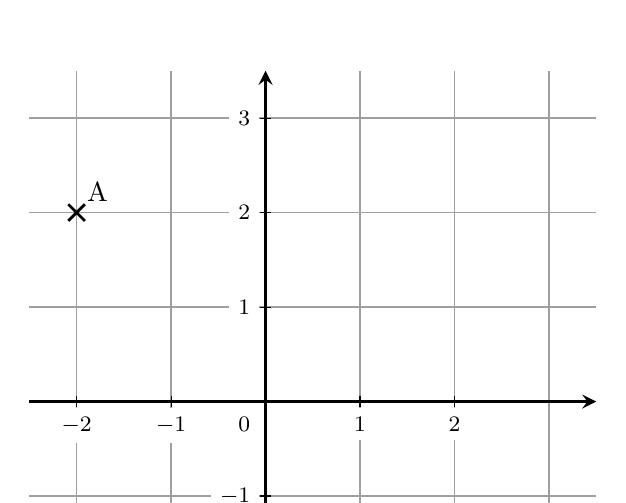
\begin{tikzpicture}[x=12mm,y=12mm,baseline={(y.base)},>=stealth]
	\draw [color = gray!75, line width = 0.5pt, xstep=1, ystep = 1] (-2.5,-1.2) grid (3.5,3.5);
	\draw[line width=1.2pt,->] (-2.5,0) -- (3.5,0);
	\foreach \x in {-2,-1,1,2}
	\draw[shift={(\x,0)},color=black] (0pt,2pt) -- (0pt,-2pt) node[below, fill = white] {\footnotesize $\np{\x}$};
	\draw[line width=1.2pt,->] (0,-1.2) -- (0,3.5);
	\foreach \y in {-1,1,2,3}
	\draw[shift={(0,\y)},color=black] (2pt,0pt) -- (-2pt,0pt) node[left, fill = white] (y) {\footnotesize $\np{\y}$};
	\draw[color=black] (-2pt,-2pt) node[below left] {{\footnotesize 0}};
	\draw[shift={(-2,2)},line width=1pt] (3pt,3pt) -- (-3pt,-3pt)
	(-3pt,3pt) -- (3pt,-3pt) (0,0) node[above right] {A};
\end{tikzpicture} \hfill~
%Fin tikz
%%Début PSTricks
%\psset{unit=1cm,arrowsize=2pt 3}
%\begin{pspicture*}(-2.5,-1.1)(2.5,3.5)
%	\psaxes[linewidth=1.25pt,labelFontSize=\scriptstyle]{->}(0,0)(-2.5,-1.1)(2.5,3.5)
%	\psgrid[gridlabels=0,subgriddiv=1,gridwidth=0.2pt](-3,-1.)(3,4)
%	\psdots(-2,2)\uput[ul](-2,2){A}
%\end{pspicture*}
%%Fin PSTricks

\medskip

\begin{minipage}[b]{0.55\linewidth}
\subsection*{Question 2}
	Dans le quadrillage ci-contre, quel est le symétrique du point K par la symétrie centrale de centre O ?
\end{minipage}\hfill~
%Début tikz
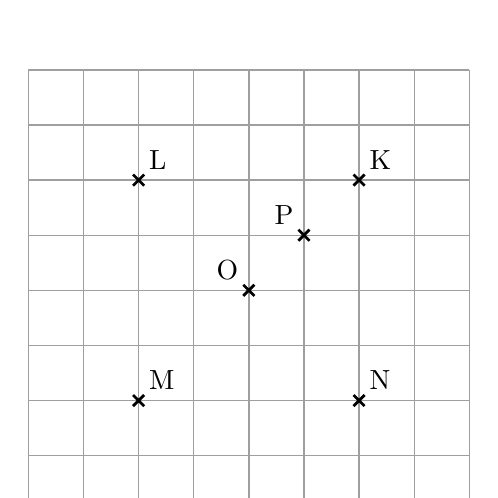
\begin{tikzpicture}[x=7mm,y=7mm,baseline={(current bounding box.center)}]
	\draw [color = gray!75, line width = 0.5pt, xstep=1, ystep = 1] (0,0) grid (8,8);
	\foreach \coordonnees/\nom/\pos in
	{{(6,6)}/K/{above right},
	{(2,2)}/M/{above right},
	{(6,2)}/N/{above right},
	{(2,6)}/L/{above right},
	{(4,4)}/O/{above left},
	{(5,5)}/P/{above left}}
		{\draw[shift=\coordonnees,line width=1pt] (2pt,2pt) -- (-2pt,-2pt)
			(-2pt,2pt) -- (2pt,-2pt) (0,0) node[\pos] {\nom};}
\end{tikzpicture}\hfill~
%Fin tikz
%%Début PSTricks
%\begin{minipage}{0.3\linewidth}
%	\psset{unit=0.5cm}
%	\begin{pspicture}(8,8)
%		\psgrid[gridlabels=0pt,subgriddiv=1,gridwidth=0.5pt]
%		\psdots(2,2)(2,6)(4,4)(5,5)(6,2)(6,6)
%		\uput[ul](2,2){M}\uput[ul](2,6){L}\uput[ul](4,4){O}\uput[ul](5,5){P}\uput[ul](6,6){K}
%	\end{pspicture}
%\end{minipage}
%%Fin PSTricks


\medskip

\begin{minipage}[t]{0.55\linewidth}
\subsection*{Question 3}
	On souhaite connaitre l'aire du triangle ABC représenté ci-contre.

	Quel calcul doit-on effectuer ?

	\begin{tblr}{colspec = {*2{X}}}
		\textbf{A.}\quad AB + BC + AC &
		\textbf{B.}\quad AC $\times$ BD $\div$ 2\\
		\textbf{C.}\quad AB $\times$ BC $\times$ CA	&
		\textbf{D.}\quad AC $\times$ BD	\\
	\end{tblr}
\end{minipage}\hfill~
%%Début tikz
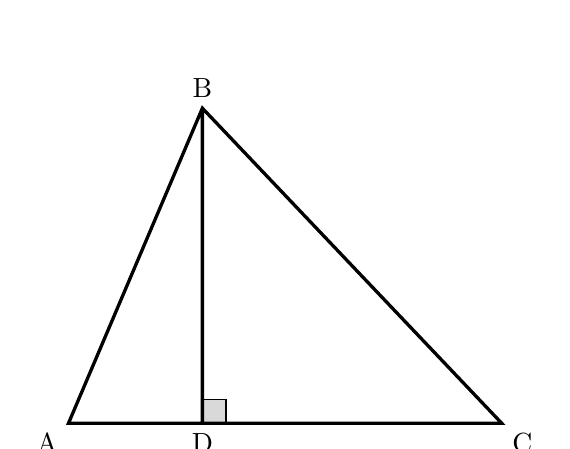
\begin{tikzpicture}[baseline={(B.base)}]
	\draw[fill=gray!30] (0,0) rectangle (0.3,0.3) ;
	\draw[line width=1.2pt]
	(-1.7,0) node[below left] {A}--
	(0,4)    node[above] (B)  {B}--
	(3.8,0)  node[below right]{C}--cycle
	(0,0)    node[below ]     {D}--(0,4);
\end{tikzpicture}
%%Fin tikz
%%%Début PSTricks
%\begin{minipage}{0.35\linewidth}
%	\psset{unit=0.9cm}
%	\begin{pspicture}(5.8,4.3)
%		\pspolygon(1.7,3.9)(0.3,0.3)(5.3,0.3)(1.7,3.9)(1.7,0.3)%BACBD
%		\uput[dl](0.3,0.3){A} \uput[u](1.7,3.9){B} \uput[dr](5.3,0.3){C} \uput[d](1.7,0.3){D}
%	\end{pspicture}
%\end{minipage}
%%%Fin PSTricks

\subsection*{Question 4}
	On lance 10 fois une pièce de monnaie.

	Les résultats obtenus sont les suivants : \emph{pile, pile, face, pile, face, face, face, face, pile, face}.

	Quelle est la fréquence d'apparition de \og \emph{pile} \fg ?

	\begin{tblr}{*{4}{X}}
		\textbf{A.}\quad $\dfrac{1}{2}$ &
		\textbf{B.}\quad $\dfrac{6}{10}$ &
		\textbf{C.}\quad $\dfrac{4}{10}$ &
		\textbf{D.}\quad $\dfrac{4}{6}$ \\
	\end{tblr}

\subsection*{Question 5}
	On note $n$ un nombre entier.

	Parmi les propositions suivantes, quelle expression donne la moitié de $n$ ?

	\begin{tblr}{*{4}{X}}
		\textbf{A.}\quad $2n$ &
		\textbf{B.}\quad $n^2$ &
		\textbf{C.}\quad $n + 2$ &
		\textbf{D.}\quad $\dfrac{n}{2}$
	\end{tblr}

\subsection*{Question 6}
	Parmi les propositions suivantes, quelle durée correspond à $\dfrac{1}{10}$ d'heure ?

	\begin{tblr}{*{4}{X}}
		\textbf{A.}\quad 0,1 min &
		\textbf{B.}\quad 1 min &
		\textbf{C.}\quad 6 min &
		\textbf{D.}\quad 10 min
	\end{tblr}

\subsection*{Question 7}
	On donne la série suivante : 10 ; 10 ; 12 ; 16.

	Calculer la moyenne de cette série.

\medskip

\begin{minipage}{0.55\linewidth}
	\subsection*{Question 8}
	La figure ci-contre n'est pas en vraie grandeur. Quelle est la valeur de $x$ ?
\end{minipage}\hfill~
%Début tikz
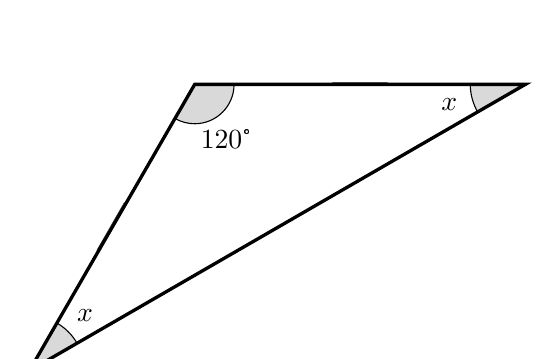
\begin{tikzpicture}[baseline={(current bounding box.center)}]
	\draw[fill=gray!30] (0,0)--(0.5,0) arc (0:-120:0.5)--cycle (-60:0.8) node{120\textdegree};
	\draw[fill=gray!30,shift={(4.2,0)}] (0,0)--(-0.7,0) arc (180:210:0.7)--cycle (195:1) node(A){$x$};
	\draw[fill=gray!30,shift={(-120:4.2)}] (0,0)--(30:0.7) arc (30:60:0.7)--cycle (45:1) node{$x$};
	\draw[line width=1.2pt] (0,0) -- (4.2,0) node[pos=0.5]{||}-- (-120:4.2)--cycle node[pos=0.5,sloped]{||};
	\end{tikzpicture}
%Fin tikz
%%Début PSTricks
%\begin{minipage}{0.37\linewidth}
%\psset{unit=0.9cm}
%\begin{pspicture}(-2,0.1)(4,-3.5)
%	\pspolygon(4;0)(0;0)(4;240)
%	\def\barre{\psline(-0.05,-0.1)(-0.05,0.1)\psline(0.05,-0.1)(0.05,0.1)}
%	\rput(2,0){\barre}\rput{60}(2;240){\barre}
%	\psarc(0;0){0.6}{-120}{0}
%	\psarc(4;240){0.4}{30}{60}\rput(-1.5,-3){$x$}
%	\psarc(4;0){0.4}{180}{210}\rput(3.35,-0.18){$x$}
%	\rput(1;-60){$120\degres$}
%\end{pspicture}
%\end{minipage}
%%Fin PSTricks

\subsection*{Question 9}

Un vélo roule à la vitesse moyenne de \np[km/h]{20}.

Quelle est la durée d'un trajet de \np[km]{15} ?

\needspace{10\baselineskip}
% saut de page si moins de 10 lignes disponibles
\section*{\hfill~ DEUXIÈME PARTIE (14 pts)\hfill~}

\section*{Exercice 1 (4 points)}

\begin{minipage}{0.45\linewidth}
	Sur la figure ci-contre, qui n'est pas représentée en vraie grandeur :
	\begin{itemize}
		\item A est le point d'intersection des droites (BE) et (TM);
		\item le triangle ABM est rectangle en A ;
		\item AT = 2,2 m; MT = 7,7 m;
		\item AE = 1,92m et MB = 7,3 m.
	\end{itemize}
\end{minipage}\hfill~
%Début tikz
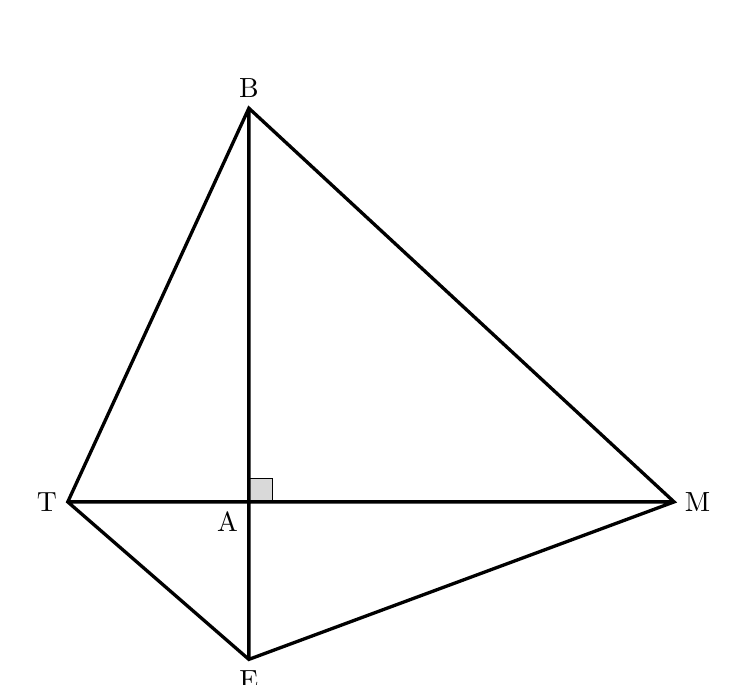
\begin{tikzpicture}[baseline={(current bounding box.center)}]
	\draw[fill=gray!30] (0,0) rectangle (0.3,0.3) ;
	\draw[line width=1.2pt]
	(0,5)    node[above](B){B}--
	(-2.3,0) node[left] {T}--
	(0,-2)   node[below]{E}--
	(5.4,0)  node[right]{M}--cycle
	(-2.3,0)--(5.4,0)
	(0,-2)--(0,5)
	(0,0)    node[below left] {A};
\end{tikzpicture}
%Fin tikz
%%%Début PSTricks
%\begin{minipage}{0.47\linewidth}
%	\psset{unit=0.8cm}
%	\begin{pspicture}(0,-2.3)(6.2,5)
%		\pspolygon(2.3,5.6)(0.2,0)(2.3,-1.8)(7.6,0)(2.3,5.6)(2.3,-1.8)(7.6,0)(0.2,0)%BTEBMT
%		\psframe(2.3,0)(2.55,0.25)
%		\uput[u](2.3,5.6){B} \uput[l](0.2,0){T} \uput[d](2.3,-1.8){E} \uput[dl](2.3,0){A} \uput[r](7.6,0){M}
%	\end{pspicture}
%\end{minipage}
%%%Fin PSTricks
\medskip

\begin{enumerate}
	\item Justifier que AM = 5,5~m.

	\item Montrer que la longueur AB est égale à 4,8~m.

	\item Calculer la mesure de l'angle $\widehat{\text{ABM}}$. Donner la valeur arrondie au degré.

	\item Montrer que les droites (TE) et (BM) sont parallèles.

	\textit{Détailler la réponse en précisant la démarche.}

	\item Le triangle ABM est l'image du triangle AET par une homothétie de centre A.

	Choisir le rapport de cette homothétie parmi les propositions suivantes. Aucune justification n'est demandée.

	\begin{center}
		\begin{tabular}{|c|c|c|}
			\hline
			\textbf{Proposition 1} & \textbf{Proposition 2} & \textbf{Proposition 3} \\
			\hline
			2,5 & $-0,4$ & $-2,5$ \\
			\hline
		\end{tabular}
	\end{center}
\end{enumerate}

\needspace{15\baselineskip}
\section*{Exercice 2 (4 points)}

On considère le programme de calcul ci-dessous.

\begin{center}
	\fbox{
		\begin{minipage}{0.55\linewidth}
			\centering \textbf{Programme A}
			\begin{itemize}[label=$\bullet~$]
				\item Choisir un nombre
				\item Soustraire 2
				\item Multiplier par 5
				\item Ajouter le triple du nombre de départ
			\end{itemize}
		\end{minipage}
	}
\end{center}

\begin{enumerate}
	\item Vérifier qu'en choisissant 1 comme nombre de départ, on obtient $-2$ avec ce programme de calcul.

	\item On note $x$ le nombre choisi au départ.
	\begin{enumerate}
		\item Montrer que le résultat du programme est $8x - 10$.

		\item Quel nombre de départ faut-il choisir pour que le résultat du programme soit égal à 0 ?
	\end{enumerate}

	\item \emph{Question d'algorithmique}
	\begin{enumerate}
		\item On considère ci-dessous le programme de calcul B, réalisé avec le logiciel \og Scratch \fg.

		\begin{center}
			%\fbox{
				%\begin{minipage}{0.6\linewidth}
				\centering \textbf{Programme B}\\[6pt]

				\begin{scratch}
					\blockinit{Quand \greenflag est cliqué}
					\blocksensing{demander \ovalnum{choisir un nombre} et attendre}
					\blockvariable{mettre \selectmenu{résultat} à \ovaloperator{\ovalnum{4}*\ovalvariable{réponse}}}
					\blockvariable{mettre \selectmenu{résultat} à \ovaloperator{\ovalvariable{résultat} - \ovalnum{5}}}
					\blockvariable{mettre \selectmenu{résultat} à \ovaloperator{\ovalnum{2} *\ovalvariable{résultat}}}
					\blocklook{dire \ovalvariable{résultat}}
				\end{scratch}
				%\end{minipage}
				%}
		\end{center}

		En appliquant ce programme de calcul au nombre 1, quel résultat final obtient-on ?

		\item Montrer que le résultat du programme A est toujours le même que celui du programme B quel que soit le nombre choisi au départ.
	\end{enumerate}
\end{enumerate}

\needspace{10\baselineskip}
\section*{Exercice 3 (4 points)}

Un centre de loisirs organise pour les jeunes d'une commune des activités pendant les vacances.

Pour s'inscrire dans ce centre de loisirs, plusieurs tarifs sont proposés :
\begin{itemize}
	\item Tarif A : on paie 5,50~\euro{} par demi-journée passée dans le centre de loisirs ;
	\item Tarif B : on paie un abonnement annuel de 15~\euro{} puis 3,50~\euro{} pour chaque demi-journée passée dans le centre ;
	\item Tarif C : on paie un forfait annuel de 64~\euro{} donnant accès à autant de demi-journées que l'on veut.
\end{itemize}

\begin{enumerate}
	\item Quel est le prix pour 12 demi-journées avec le tarif B ?
	\item On désigne par $x$ le nombre de demi-journées passées dans le centre de loisirs.
	On considère les trois fonctions $f,\, g$, et $h$ suivantes :

	\[f : x \longmapsto 15 + 3,5x \qquad\qquad g : x \longmapsto 64 \qquad\qquad h : x \longmapsto 5,5x\]

	Sans justifier, associer chacune de ces fonctions au tarif qu'elle représente.

	\item Le graphique ci-dessous représente les fonctions $f,\, g$, et $h$.
	Sans justifier, associer à chaque représentation graphique ($d_1$), ($d_2$) et ($d_3$) la fonction $f$, $g$ ou $h$ correspondante.

	\begin{center}
		%Début Tikz
		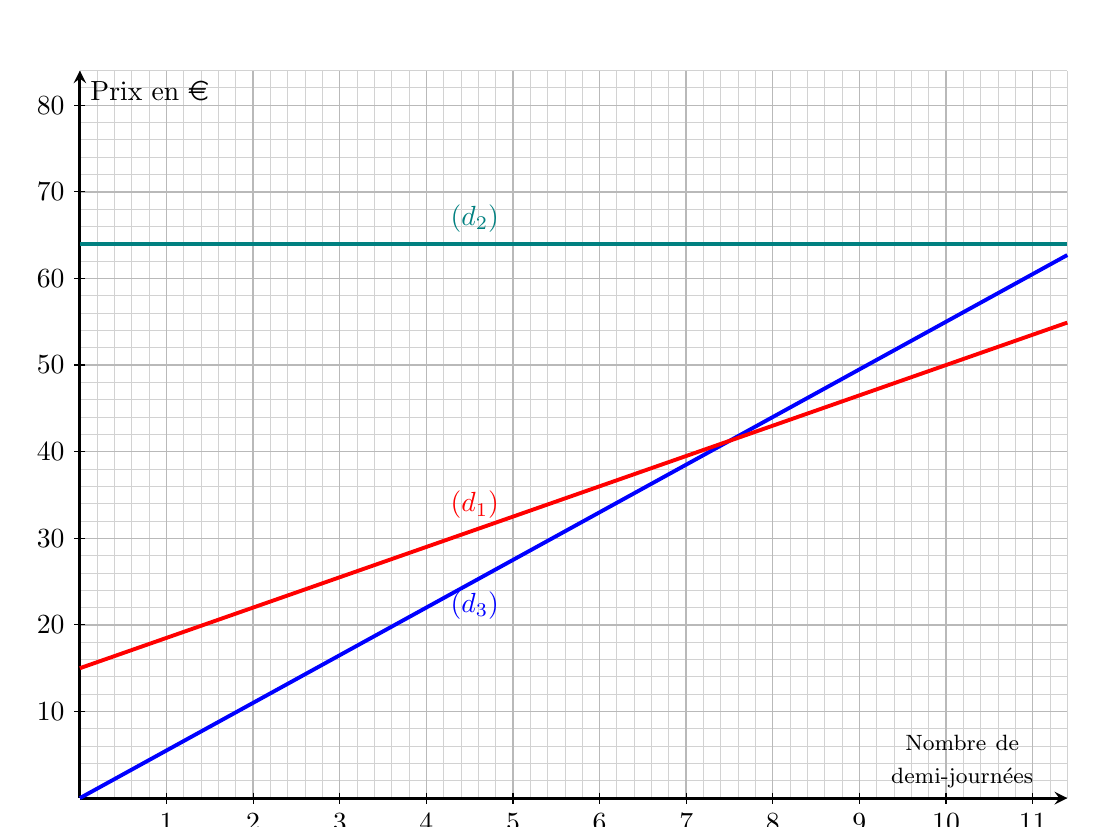
\begin{tikzpicture}[x=11mm, y=1.1mm, >=stealth]
		\draw[color = gray!35, line width = 0.3pt, xstep=0.2, ystep = 2] (0,0) grid (11.4,84);
		\draw[color = gray!55, line width = 0.5pt, xstep=1, ystep = 10] (0,0) grid (11.4,84);
		\draw[->,line width=1pt] (0,0) -- (11.4,0) node[above left,text width=2.4cm,align = center] {\footnotesize Nombre de demi-journées};
		\draw[->,line width=1pt] (0,0) -- (0,84) node[below right] {Prix en \euro{}};
		\foreach \x in {1,...,11}
			\draw (\x,2pt) -- (\x,-2pt) node[below] {\np{\x}};
		\foreach \y in {10,20,...,80}
			\draw (2pt,\y) -- (-2pt,\y) node[left] {\np{\y}};
		\draw[teal,line width=1.4pt] (0,64) -- (11.4,64) node[pos=0.4,above]{$(d_2)$};
		\draw[blue,line width=1.4pt] (0,0) -- (11.4,62.7) node[pos=0.4,below]{$(d_3)$};
		\draw[red,line width=1.4pt] (0,15) -- (11.4,54.9)
		node[pos=0.4,above]{$(d_1)$};
		\end{tikzpicture}
		%Fin Tikz
%		%Début PSTricks
%		\psset{xunit=1cm,yunit=0.1cm,arrowsize=2pt 3}
%		\begin{pspicture}(-0.6,-5)(11,85)
%			\psaxes[linewidth=1.25pt,Dy=10,labelFontSize=\scriptstyle]{->}(0,0)(0,0)(11,85)
%			\multido{\n=0+1}{12}{\psline[linewidth=0.15pt](\n,0)(\n,85)}
%			\multido{\n=0+10}{9}{\psline[linewidth=0.15pt](0,\n)(11,\n)}
%			\psplot[plotpoints=2000,linewidth=1.25pt,linecolor=red]{0}{11}{3.5 x mul 15 add}
%			\psplot[plotpoints=2000,linewidth=1.25pt,linecolor=blue]{0}{11}{5.5 x mul}
%			\psline[linewidth=1.25pt,linecolor=green](0,64)(11,64)
%			\uput[u](9,0){\footnotesize Nombre de demi-journées}
%			\uput[r](0,83){\footnotesize Prix en \euro}
%			\rput(3,14){\blue $(d_3)$}\rput(3,30){\red $(d_1)$}\rput(3,66){\green $(d_2)$}
%		\end{pspicture}
		%Fin PSTricks
	\end{center}

	\item La droite ($d_1$) représente-t-elle une situation de proportionnalité ?

	\textit{Détailler la réponse en précisant la démarche.}

	\item Lire graphiquement le nombre de demi-journées à partir duquel le tarif B devient plus avantageux que le tarif A. Aucune justification n'est demandée.

	\needspace{10\lineskip}
	\item On a réalisé dans un tableur le tableau de valeurs correspondant au tarif B suivant le nombre de demi-journées de présence.

	\begin{tblr}{hlines, vlines, colsep=1pt,
			colspec={*{18}{X}},
			columns={c,font=\sffamily},	rows={m},
			cell{2-Z}{2-Z}={font=\small \sffamily},
			row{1}={rowsep=0pt,ht=7mm, bg=gray9},
			column{1}={colsep=0pt,7mm,bg=gray9},
			column{2}={2.8cm},
			cell{1}{1}={gray9,halign=r,valign=b,cmd={\tikz[baseline={(0,0.15)}]{\clip(0,0) rectangle (0.6,0.5) ;\fill[gray!50] (0,0)--(0.5,0.5)--(0.5,0);}}}
			}
		  & A                                   & B    & C  & D    & E  & F    & G  & H    & I  & J    & K  & L    & M  & N    & O  & P    & Q   \\
		1 & Nombre de demi-journées d'activités & 1    & 2  & 3    & 4  & 5    & 6  & 7    & 8  & 9    & 10 & 11   & 12 & 13   & 14 & 15   & 16  \\
		2 & Tarif B en \euro                    & 18,5 & 22 & 25,5 & 29 & 32,5 & 36 & 39,5 & 43 & 46,5 & 50 & 53,5 & 57 & 60,5 & 64 & 67,5 & 71
	\end{tblr}

	\begin{enumerate}
		\item Parmi les trois formules proposées ci-dessous, recopier celle qui a été saisie dans la cellule \textsf{B2}, puis étirée vers la droite pour compléter le tableau.

		\begin{center}
			\begin{tblr}{colspec={*{3}{X[c,font=\sffamily]}},hlines, vlines}
				=15+3,5*$x$ & =15+3,5*1 & =15+3,5*B1 \\
			\end{tblr}
		\end{center}

		\item En utilisant le tableau de valeurs ci-dessus, déterminer le nombre de demi-journées à partir duquel le tarif C devient plus avantageux que le tarif B. Aucune justification n'est demandée.
	\end{enumerate}
\end{enumerate}

%---------------------------------------------------------
% Fin du document
%---------------------------------------------------------
\end{document}